\begin{appendix}

% ================================================================
\chapter{Architecture Diagrams} \label{appendix:architectures}
% ================================================================
This appendix provides the complete structural diagrams for the deep learning architectures utilised in this thesis.

\begin{figure}[htbp]
    \centering
    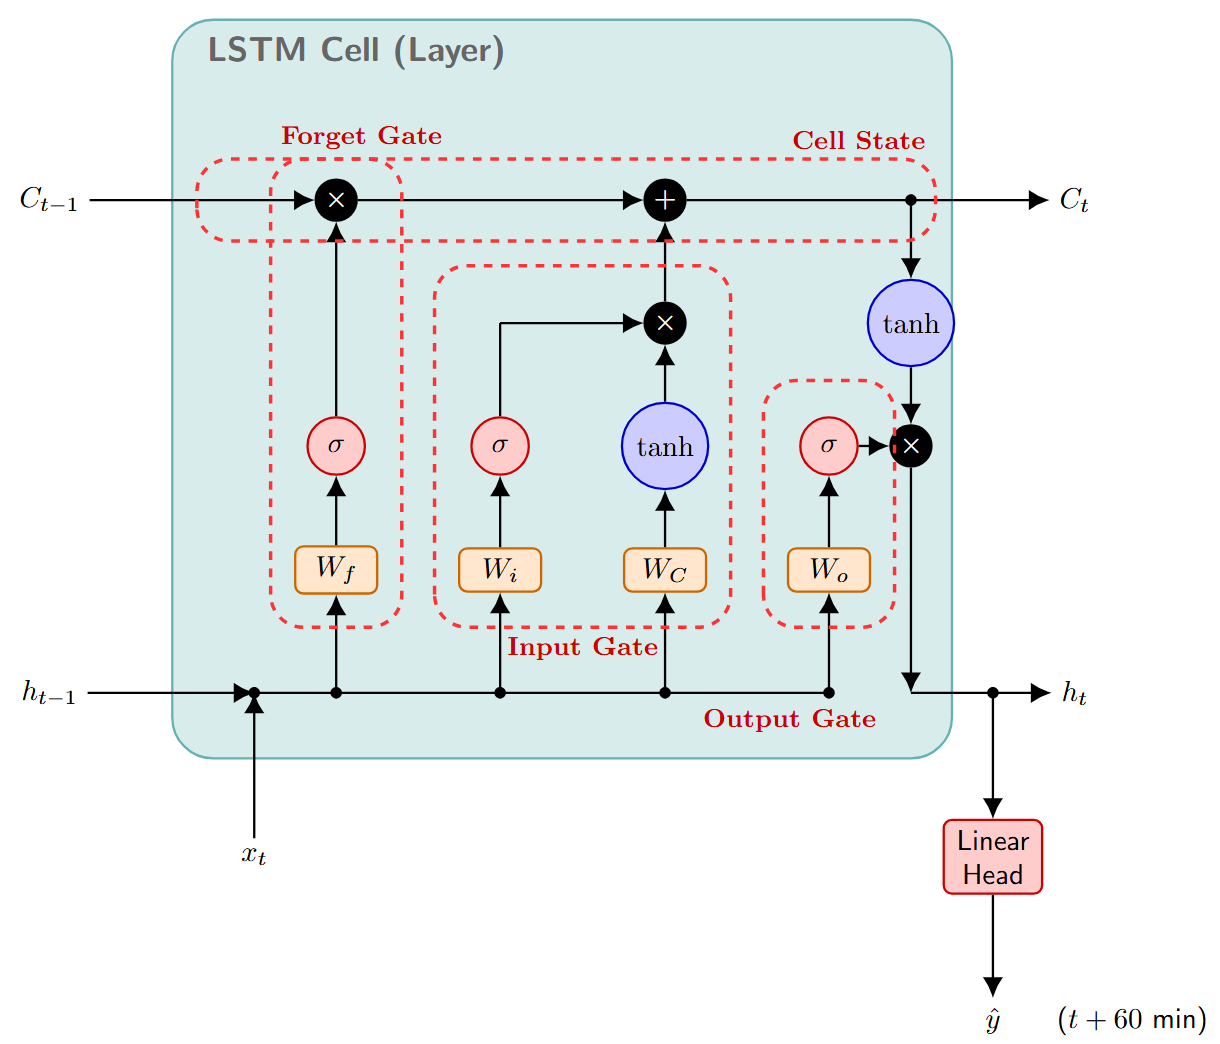
\includegraphics[width=0.9\textwidth]{lstm_cell.png}
    \caption[Architecture of the LSTM model]{Architecture of the LSTM model used as the recurrent baseline. The input is a 24-step lookback window representing 120~minutes of CGM data.}
    \label{fig:app:lstm_arch}
\end{figure}

\begin{figure}[htbp]
    \centering
    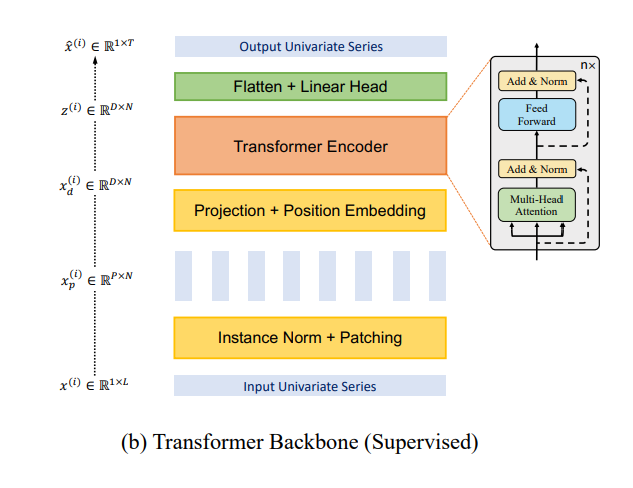
\includegraphics[width=0.9\textwidth]{patchtst_arch_b.png}
    \caption[Architecture of the PatchTST model]{Architecture of the PatchTST model adapted to the CGM setting, incorporating Reversible Instance Normalisation (RevIN).}
    \label{fig:app:patchtst_arch}
\end{figure}


% ================================================================
\chapter{Supplementary Evaluation Figures} \label{appendix:detailed_metrics}
% ================================================================
This appendix contains supplementary figures that support the findings presented in Chapter~\ref{ch:experiments}.

\begin{figure}[htbp]
    \centering
    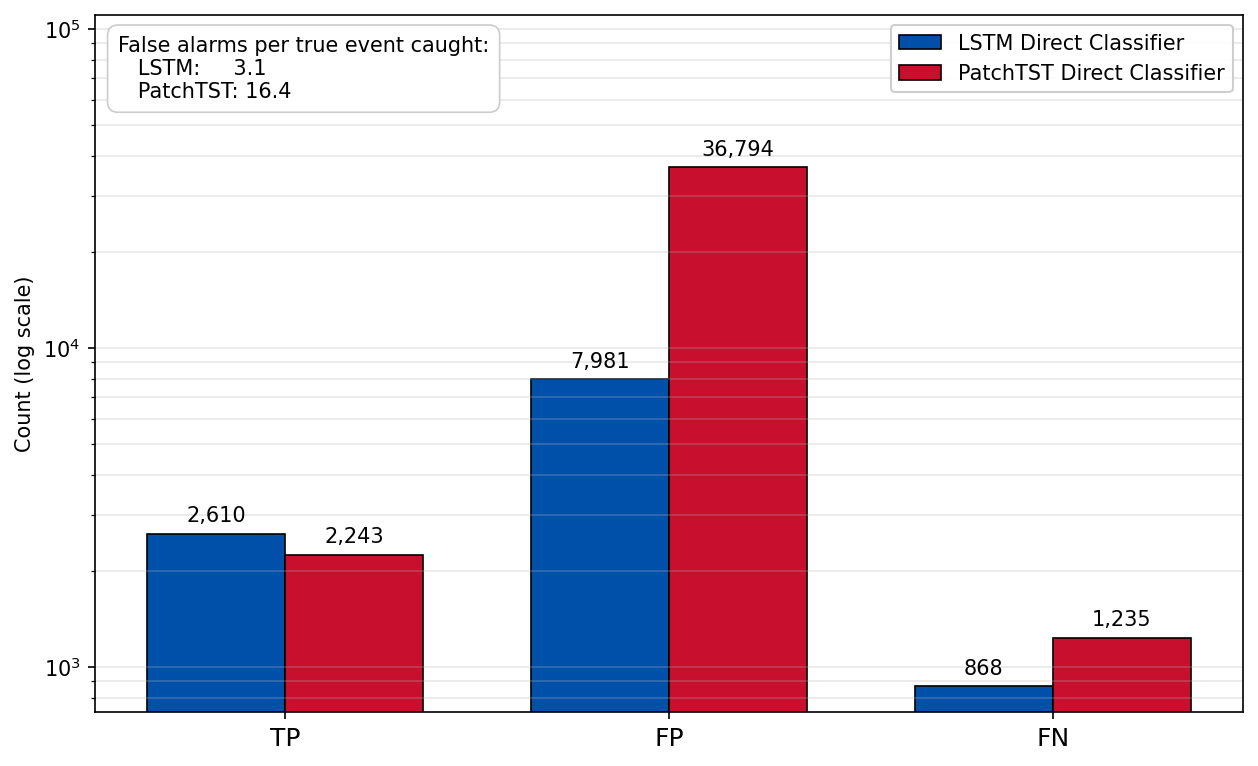
\includegraphics[width=0.85\textwidth]{confusion_counts.png}
    \caption[Confusion counts for direct event classifiers]{Absolute confusion counts (TP, FP, FN; log scale) for the LSTM and PatchTST direct event classifiers evaluated on Task~A across the full 36-patient cohort. The LSTM accumulates 3.1 false alarms per true positive detected; the PatchTST incurs 16.4 false alarms per true positive, reflecting its substantially lower precision despite comparable recall (Table~\ref{tab:exp:classifiers} in Chapter~\ref{ch:experiments}).}
    \label{fig:app:confusion_counts}
\end{figure}

\begin{figure}[htbp]
    \centering
    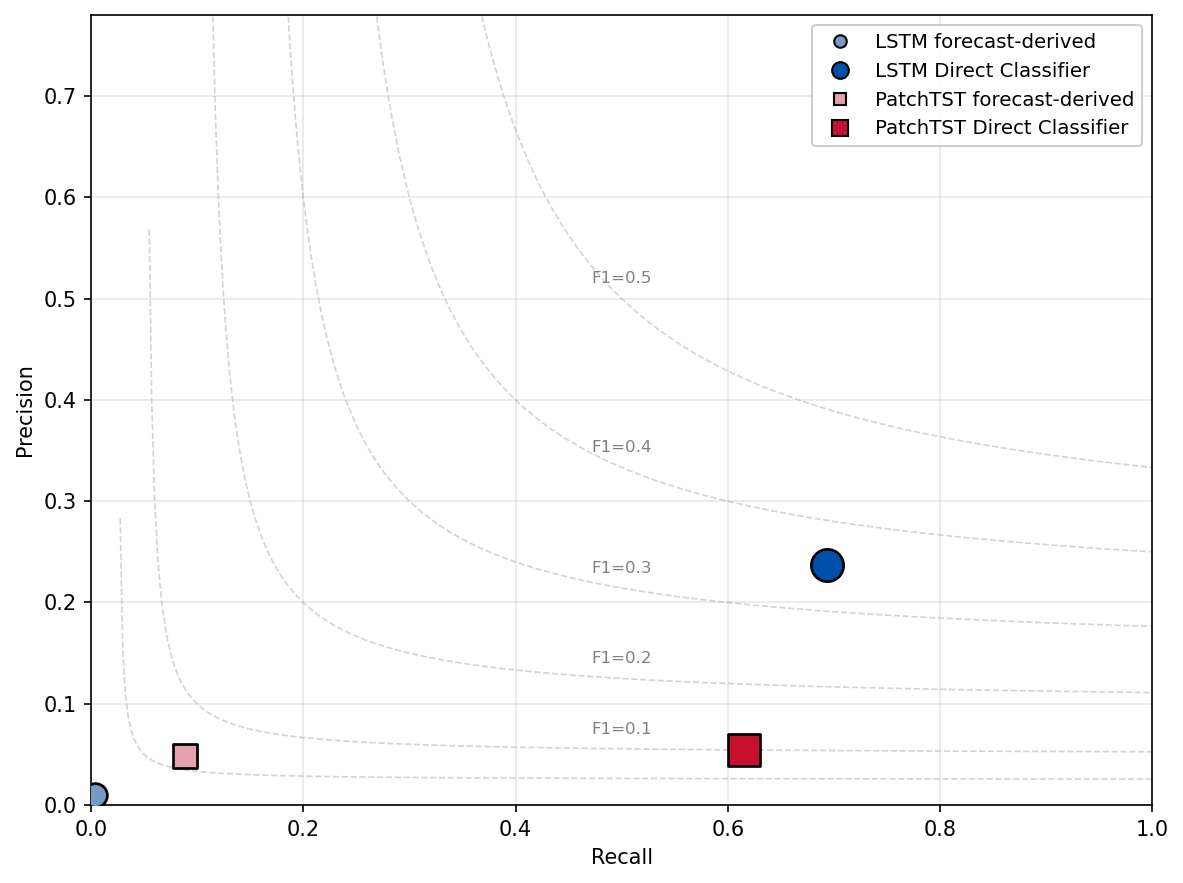
\includegraphics[width=0.9\textwidth]{pr_paradox.png}
    \caption[Precision--Recall space: forecast-derived vs.\ direct classifiers]{Precision--Recall space for forecast-derived detectors (hollow markers) and direct binary classifiers (filled markers) for LSTM (circles) and PatchTST (squares). The forecast-derived detectors cluster near the origin due to the systematic prediction delay. Direct training on the classification task dramatically shifts both models into clinically relevant recall regimes, with the LSTM achieving the superior precision--recall trade-off.}
    \label{fig:app:pr_paradox}
\end{figure}

\begin{table}[htbp]
\centering
\small
\caption[$\tau$-sweep numerical breakdown]{Detailed numerical breakdown of the forecast-derived hypoglycaemia detection performance as a function of the tolerance window $\tau$ (in minutes) for the LSTM and PatchTST MSE baselines. Metrics are computed over the full 36-patient cohort. The monotonic increase of all metrics with $\tau$ confirms that performance gains reflect tolerance compensation for the static prediction delay rather than genuine anticipatory detection.}
\label{tab:app:tau_sweep}
\begin{tabular}{lrrrr}
\toprule
Model / $\tau$ & Precision\,$\uparrow$ & Recall\,$\uparrow$ & F1\,$\uparrow$ & F2\,$\uparrow$ \\
\midrule
\multicolumn{5}{l}{\textit{LSTM (MSE baseline)}} \\[2pt]
 5 min   & 0.007 & 0.002 & 0.004 & 0.003 \\
 10 min  & 0.010 & 0.004 & 0.005 & 0.004 \\
 15 min  & 0.010 & 0.004 & 0.005 & 0.004 \\
 20 min  & 0.010 & 0.004 & 0.005 & 0.004 \\
 25 min  & 0.010 & 0.004 & 0.005 & 0.004 \\
 30 min  & 0.019 & 0.007 & 0.011 & 0.008 \\
 35 min  & 0.067 & 0.017 & 0.025 & 0.019 \\
 40 min  & 0.081 & 0.018 & 0.029 & 0.021 \\
 45 min  & 0.088 & 0.024 & 0.035 & 0.027 \\
 50 min  & 0.129 & 0.040 & 0.058 & 0.046 \\
 55 min  & 0.169 & 0.053 & 0.076 & 0.060 \\
 60 min  & 0.230 & 0.082 & 0.113 & 0.092 \\
\midrule
\multicolumn{5}{l}{\textit{PatchTST (MSE baseline)}} \\[2pt]
 5 min   & 0.020 & 0.571 & 0.037 & 0.079 \\
 10 min  & 0.024 & 0.592 & 0.044 & 0.092 \\
 15 min  & 0.027 & 0.599 & 0.050 & 0.104 \\
 20 min  & 0.031 & 0.606 & 0.056 & 0.115 \\
 25 min  & 0.034 & 0.612 & 0.062 & 0.125 \\
 30 min  & 0.037 & 0.615 & 0.067 & 0.134 \\
 35 min  & 0.040 & 0.620 & 0.073 & 0.143 \\
 40 min  & 0.043 & 0.621 & 0.077 & 0.151 \\
 45 min  & 0.046 & 0.622 & 0.082 & 0.158 \\
 50 min  & 0.049 & 0.619 & 0.086 & 0.165 \\
 55 min  & 0.052 & 0.616 & 0.091 & 0.172 \\
 60 min  & 0.054 & 0.615 & 0.095 & 0.179 \\
\bottomrule
\end{tabular}
\end{table}


% ================================================================
\chapter{Hyperparameter Details} \label{appendix:hyperparams}
% ================================================================
This appendix specifies the final hyperparameter configuration used for all experiments. Parameters were determined via Optuna~\cite{akiba2019optuna} with 50 trials on the designated tuning patient (85202) and held constant across all three research objectives.

\begin{table}[htbp]
\centering
\caption[Optuna-tuned hyperparameters]{Optuna-tuned hyperparameters for the LSTM and PatchTST architectures. The search was conducted on the validation set of patient 85202 only. Identical hyperparameters are used for all training objectives (MSE, Bounded-Lag, Soft-DTW, Multi-Step); only the loss function or output head is modified per objective.}
\label{tab:app:hyperparams}
\begin{tabular}{lrr}
\toprule
Hyperparameter & LSTM & PatchTST \\
\midrule
Hidden size / $d_\text{model}$      & 256     & 64 \\
Number of layers                     & 2       & 3 \\
Dropout                              & 0.159   & 0.025 \\
Learning rate                        & $9.61 \times 10^{-4}$ & $1.21 \times 10^{-4}$ \\
Batch size                           & 128     & 128 \\
Feed-forward dim.\ ($d_\text{ff}$)  & ---     & 256 \\
Attention heads ($h$)                & ---     & 4 \\
Lookback window                      & \multicolumn{2}{c}{24 steps (120 min)} \\
Forecast horizon                     & \multicolumn{2}{c}{12 steps (60 min)} \\
Optuna trials                        & \multicolumn{2}{c}{50} \\
\bottomrule
\end{tabular}
\end{table}

\end{appendix}
